\chapter{Single Mode}\index{Single mode}
\label{c:single}

\tao has two \vn{modes} for entering commands. In \vn{Single Mode},
described in this chapter, each keystroke represents a command.  That
is, the user does not have to press the carriage control key to signal
the end of a command (there are a few exceptions which are noted
below). Conversely, in \vn{Line Mode}, which is described in
Chapter~\sref{c:command}, \tao waits until the \vn{return} key is
depressed to execute a command. That is, in Line Mode a command
consists of a single line of input.  Single Mode is useful for quickly
varying parameters to see how they affect a lattice but the number of
commands in Single Mode is limited.

From \vn{line mode} use the \vn{single-mode} command (\sref{s:sing})
to get into \vn{single mode}. To go back to \vn{line mode} type
"\vn{Z}".

%% key_table ------------------------------------------------------------------------
\section{Key Bindings}\index{Key Bindings}
\label{s:key.bind}

The main purpose of Single Mode is to associate certain keys with
certain variables so that the pressing of these keys will change their
associated variable. This is called a \vn{key binding}.  Key bindings
are established via the \vn{key_bindings} initialization namelist (See
Section~\sref{s:init.key.bind}). The variables are divided into banks of
10. The 0\Th bank uses variables \vn{key(1)} through \vn{key(10)} from
the \vn{key_bindings} namelist, the 1\St bank uses variables
\vn{key(11)} through \vn{key(20)}, etc.  

At any one time, only one bank is active. To see the status of this
bank, a \vn{key table} plot can be setup as shown in
Figure~\ref{f:key.table}. The relationship between the keys and a
change in a variable is:
\begin{example}
                 Change by factor of:          
     Variable    -10  -1    1     10
   ----------    ---  ---  ---  -------
    1 + 10*ib     Q    q    1   shift-1   ("!")
    2 + 10*ib     W    w    2   shift-2   ("@")
    3 + 10*ib     E    e    3   shift-3   ("\#")
    4 + 10*ib     R    r    4   shift-4   ("\$")
    5 + 10*ib     T    t    5   shift-5   ("%")
    6 + 10*ib     Y    y    6   shift-6   ("^")
    7 + 10*ib     U    u    7   shift-7   ("\&")
    8 + 10*ib     I    i    8   shift-8   ("*")
    9 + 10*ib     O    o    9   shift-9   ("(")
   10 + 10*ib     P    p    0   shift-0   (")")
\end{example}
In the above table ib is the bank number (0 for the 0\Th bank, etc.),
and the change is in multiples of the \vn{step} for a variable as
specified in the \vn{key_bindings} namelist. 

Initially the 0Th bank is active. The left arrow and right arrow are
used to decrease or increase the bank number.  Additionally the
"\vn{<}" and "$>$" keys can be used to change the deltas for the
variables.

For example, looking at Figure~\ref{f:key.table}, the \vn{"1:"} in
the upper left corner of the \vn{Key Table} shows that the 1\St bank
is active which corresponds to keys \vn{key(11)} through \vn{key(20)}
from the \vn{key_bindings} namelist.  Since, in this case, keys
\vn{key(19)} and \vn{key(20)} have not been defined, the corresponding
rows in the \vn{Key Table} are blank.

\vn{key(14)} is associated with the \vn{"4"} key and from the \vn{Key
Table} it is seen that the bound attribute is the \vn{b1_gradient} of
the element named \vn{Q15_2}.  Thus, if the \vn{"4"} key is depressed
in single mode, the value of the \vn{b1_gradient} of element
\vn{Q15_2} will be increased by the given Delta (0.1000 in this
case). Pressing the \vn{"r"} key (which is just below the \vn{"4"}
key) will decrease the value of the \vn{b1_gradient} by 0.1000. Using
the shift key, which is shift-4 (\vn{"\$"}) will increase
\vn{b1_gradient} by 10 times the given delta (1.000 in this case) and
\vn{"R"} will decrease by 10 time the given delta.

Since element \vn{Q15_2} is also displayed in the \vn{Lattice Layout},
there is a \vn{"4"} drawn above this element that reflects the fact
that the element contains a bound attribute. Since, in this case, the
Lattice Layout only shows part of the lattice, not all key indexes are
present.

%------------------------------------------------------------------------

\begin{figure}
  \centering
  \includegraphics[width=5in]{layout-graph-table.eps}
  \caption[Example key table with a lattice layout and data plots.]
{A lattice layout plot (top) above a data plot (middle) 
which in turn is above a key table plot (bottom). The points on the
curves in the data plot mark the edges of the elements displayed in
the lattice layout. Elements that have attributes that are varied as
shown in the key table have the corresponding key table number printed
above the element's glyph in the lattice layout.}
  \label{f:key.table}
\end{figure}

%% keys ------------------------------------------------------------------------
\section{List of Key Strokes}\index{Single Mode!List of Key Strokes}
\label{s:keys}

In the following list, certain commands use multiple key strokes. For
example, the \vn{"/v"} command is invoked by first pressing the slash
(\vn{"/"}) key followed by the \vn{"v"} key. \vn{"a $<$left_arrow$>$"}
represents pressing the \vn{"a"} key followed by the left-arrow key.

\begin{description}
\item[?]
Type a short help message.

\item[a $<$left\_arrow$>$]
Pan plots left by half the plot width.

\item[a $<$right\_arrow$>$]
Pan plots right by half the plot width.

\item[a $<$up\_arrow$>$]
Pan plots up by half the plot height.

\item[a $<$down\_arrow$>$]
Pan plots down by half the plot height.

\item[s $<$left\_arrow$>$]
Scale x-axis of plots by a factor of 2.0.

\item[s $<$right\_arrow$>$]
Scale x-axis of plots by a factor of 0.5

\item[s $<$up\_arrow$>$]
Scale y-axis of plots by a factor of 2.0.

\item[s $<$down\_arrow$>$]
Scale y-axis of plots by a factor of 0.5


\item[z $<$left\_arrow$>$]
Zoom x-axis of plots by a factor of 2.0.

\item[z $<$right\_arrow$>$]
Zoom x-axis of plots by a factor of 0.5

\item[z $<$up\_arrow$>$]
Zoom y-axis of plots by a factor of 2.0.

\item[z $<$down\_arrow$>$]
Zoom y-axis of plots by a factor of 0.5

\item[c]  
Show constraints.

\item[g]
Go run the default optimizer. The optimizer will run until you type a
'.' (a period).  Periodically during the optimization the variable
values will be written to files, one for each universe, whose name is
\vn{tao_opt_vars\#.dat}. where \vn{\#} is the universe number.

\item[v]
Show variable values in bmad compatible lattice format. See also the
\vn{/v} and \vn{\W v} commands.

\item[V] 
Same an \vn{v} except only only variables used in the optimization are printed.

\item[Z] 
Go back to \vn{line mode}

\item[$<$]
Reduce the deltas (the amount that a variable is changed when you use
the keys 0 through 9) of all the variables by a factor of 2.

\item[$>$]
Increase the deltas (the amount that a variable is changed when you
use the keys 0 through 9) of all the variables by a factor of 2.

\item[$<$left\_arrow$>$]
Shift the active key bank down by 1: ib -$>$ ib - 1

\item[$<$right\_arrow$>$]
Shift the active key bank up by 1: ib -$>$ ib + 1

\item[/$<$up\_arrow$>$]
Increase all key deltas by a factor of 10.

\item[/$<$down\_arrow$>$]
Decrease all key deltas by a factor of 10.

\item[$<$CR$>$]
Do nothing but replot.

\item[-p]
Toggle plotting. Whether to plot or not to plot is initially
determined by plot%enable.

\item['$<$command$>$]
Accept a Line Mode (\sref{c:command}) command.

\item[/e $<$Index or Name$>$]
Prints info on a lattice element. If there are two lattices being used
and only the information of an element from one particular lattice is
wanted then prepent with "n@" where n is the lattice
index.

\item[/l]
Print a list of the lattice elements with Twiss parameters.

\item[/u $<$Universe Index$>$]
Switch the viewed universe.

\item[/v]
Write variable values to the default output file.  The default output
file name is set by \vn{global%var_out}. This file is in BMAD
format. See also the \vn{V} command.

\item[/x $<$min$>$ $<$max$>$]
Set the horizontal scale (longitudinal position) min and max values
for all the plots. This is the same as setting p%x%min and p%x%max in
the \tao input file. If \vn{min} and \vn{max} are not given then the scale
will be choisen to include the entire lattice. 

\item[/y $<$min$>$ $<$max$>$]
Set the y-axis min and max values for all the plots. This is the same
as setting p%y%min and p%y%max in the \tao input file. If \vn{min} and
\vn{max} are not given then an autoscale will be done.

\item[=v $<$digit$>$ $<$value$>$]
Set variable value. \vn{<digit>} is between 0 and 9 corresponding to a
variable of the current bank. \vn{<value>} is the value to set the
variable to.

\item[=$<$right\_arrow$>$]
Set saved ("value0") values to variable values to saved values. The
saved values (the value0 column in the display) are initially set to
the initial value on startup. There are saved values for both the
manual and automatic variables. Note that reading in a TOAD input file
will reset the saved values. If you want to save the values of the
variables in this case use "/w" to save to a file. Use the
"\vn{/$<$left_arrow$>$}" command to go in the reverse direction.

\item[=$<$left\_arrow$>$]
Paste saved ("value0") values back to the variable values.  The saved
values (the value0 column in the display) are initially set to the
initial value on startup. Use the "\vn{/$<$right_arrow$>$}" command to go in
the reverse direction.

\end{description}
